\subsection{Problema a resolver}
El siguiente ejercicio consiste en exponer un algoritmo capaz de devolver, dado un conjunto de intervalos, el subconjunto máximo de los que no se solapan entre sí. Luego, el algoritmo debe poder tomar las fechas ofrecidas por los profesores del programa de Profesores Visitantes de la FCEyN para sus cursos e indicar qué cursos deberían elegirse para maximizar la cantidad de éstos en el ciclo. Cada intervalo corresponde a la fecha en que un profesor dictará su curso. El primer elemento del intervalo corresponde a la fecha de inicio y el segundo a la fecha de fin, siendo siempre la de fin mayor o igual a la de inicio. Para la simplificación del manejo de los datos, éstos se representan con números enteros positivos.\newline
\newline
\textbf {Formatos de entrada y salida:}\newline
\newline
La entrada contiene varias instancias del problema. Cada instancia consta de una línea con el siguiente formato:

$$n\ i_{1}\ f_{1}\ i_{2}\ f_{2}\ ...\ i_{n}\ f_{n}$$


donde \textbf{$n$} es la cantidad de cursos ofrecidos por los profesores (numerados de 1 a n) y los valores \textbf{$[i_{1},f_{1}],\ ...,\ [i_{n},f_{n}]$} representan los días de inicio y fin de cada uno de los n cursos. Todos los datos son enteros positivos. La entrada concluye con una línea comenzada por \# que no debe ser procesada.\newline

La salida debe contener una línea por cada instancia de entrada, donde se listan los números de los cursos elegidos para el ciclo de cursos.\newline
\newline
En lo que sigue, presentaremos dos ejemplos sobre cómo debería comportarse nuestro algoritmo:\newline

{\large{\textbf{Ejemplos:}}}\newline

\begin{figure}[H] %[h] Aqui [b] para button [t] para top
\begin{center}
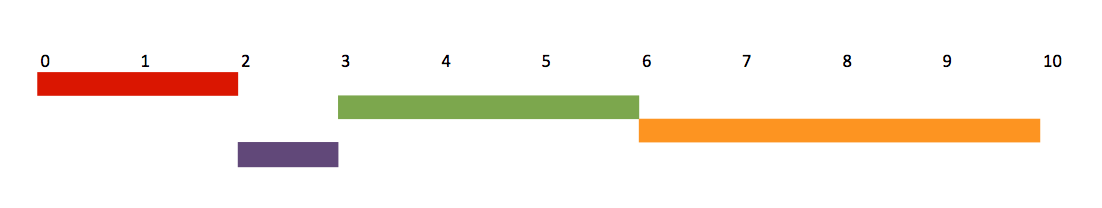
\includegraphics[width=460pt]{../imgs/ejemplo1ej2.png}
\end{center}
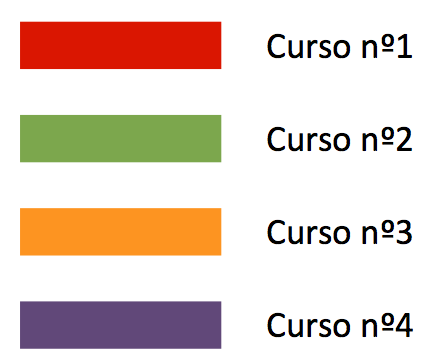
\includegraphics[width=90pt]{../imgs/leyendaej2.png}
\caption{Ejemplo 1.}
\end{figure}

\textbf{Formato de entrada:} $$3\ \ 0\ \ 1\ \ 3\ \ 5\ \ 6\ \ 9$$

\textbf{Formato de salida:} $$1\ \ 2\ \ 3$$


\begin{figure}[H] %[h] Aqui [b] para button [t] para top
\begin{center}
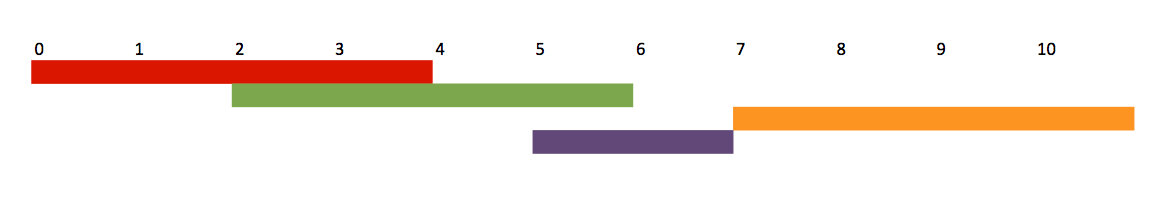
\includegraphics[width=480pt]{../imgs/ejemplo2ej2.png}
\end{center}
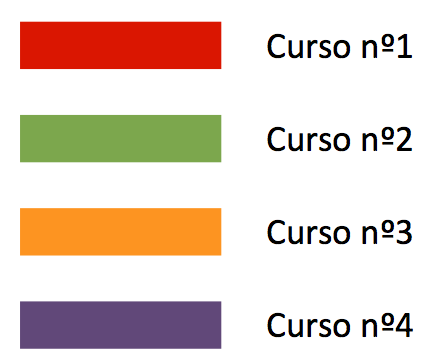
\includegraphics[width=90pt]{../imgs/leyendaej2.png}
\caption{Ejemplo 2.}
\end{figure}


\subsection{Resolución coloquial}
Decidimos resolver el problema ordenando los cursos de acuerdo a la fecha de finalización de los mismos por orden creciente. De este modo, se recorrió cada intervalo correspondiente a cada curso y, cuando el $i-ésimo$ no se solapaba con el anterior, se lo agregaba a la solución.\newline

Al analizar el problema a resolver, nos percatamos de que el algoritmo de maximización de intervalos no solapados corresponde a un $algoritmo\ goloso$. El pseudocódigo que describe el algoritmo es el siguiente:\newline


\begin{algorithm}[H]
	\SetAlgoLined
	\caption{MaximaCantidadDeIntervalosNoSolapados}
	\KwIn{Cursos $CS$}
	\KwOut{listaDeCursos}
	\eIf{\#CS == 0}{
		\textbf{devolver} $ListaVacia$\\
	}{
		$CS$ = OrdenarPorFin($CS$)\\
		Lista res = filtrarSolapamientos($CS$)\\
		\textbf{devolver} \#res ++ ordenar(res)\\
	}
\end{algorithm}

\begin{algorithm}[H]
	\SetAlgoLined
	\caption{filtrarSolapamientos}
	\KwIn{Cursos $CS$}
	\KwOut{listaDeCursos}
	Curso $anterior$ = Primer curso de $CS$\\
	Lista $res$\\
	\For{Curso $c$ en $CS$}{
		\If{$c$ no se solapa con $anterior$}{
			$anterior$ := $c$\\
			$res \leftarrow c$
		}
	}
	\textbf{devolver} $res$\\	
\end{algorithm}

donde $Cursos$ es una secuencia conteniendo la información (fecha de inicio y de fin) de los cursos del ciclo. $ordenarPorFin$ es un algoritmo que toma los cursos y los ordena de acuerdo a su fecha de finalización. Por último, "no se solapa" verifica que la fecha de inicio del intervalo que se quiere agregar no se superponga con la fecha de fin del agregado precedentemente\\
Una observacion que hicimos:\\
O1: Los dias de inicio son menores a los dias de finalizacion de cada curso.\\

\textbf{Modelo formal:}\\
Sea $v$ un intervalo, este intervalo está representado por dos valores: $v_{i}$ es el inicio del intervalo y $v_{f}$ es el fin del intervalo. Sea C un conjunto de intervalos. Nuestro modelo del problema mapea a los cursos como intervalos, donde el dia de incio es el valor $v_{i}$ y el dia de finalizacion del curso es $v_{f}$, la solucion se obtiene encontrando un conjunto maximo de elementos cuyos intervalos no se solapen, esto significa: 
\par{$$\forall v^{1}, v^{2} \in C, v^{1} \neq v^{2}\ | \ (v^{1}_{f} < v^{1}_{i}) \vee (v^{2}_{f} < v^{1}_{i})$$} 
esta es condición suficiente ya que por O1 el valor de incio de un curso es menor al valor de fin del mismo curso para todos los cursos.

\subsection{Demostración de correctitud}

Veamos que, efectivamente, nuestro algoritmo encuentra una solución óptima $S$ cuya cantidad de intervalos es $k$. Para ello, vamos a suponer que tenemos la salida ordenada por la fecha de fin de cada intervalo. Supongamos que existe una solución óptima $S'$ cuya cantidad de intervalos es $n$, dicha solución se encuentra ordenada del mismo modo que $S$.\\ Sean $S_{1}$ y $S'_{1}$ los primeros intervalos de ambas soluciones. En el caso en el que $f_{S_{1}} \leq f_{S'_{1}}$, se puede reemplazar $S'_{1}$ por $S_{1}$ pues, si $S'_{2}$ no se solapa con $S'_{1}$, tampoco lo hará con $S_{1}$. El caso $f_{S'_{1}} < f_{S_{1}}$ no puede ocurrir pues nuestro algoritmo selecciona el intervalo cuya fecha de fin es la menor.\\
Por otra parte, si consideramos $S_{2}$ y $S'_{2}$ y por el mismo criterio utilizado anteriormente, si $f_{S_{2}} \leq f_{S'_{2}}$, se puede reemplazar $S'_{2}$ por $S_{2}$ pues, si $S'_{1}$ no se solapa con $S'_{2}$, tampoco se solapará con $S_{2}$. Este mismo razonamiento puede extenderse, con el mismo principio, hasta $S_{k}$.\\
Tal como mencionado, los intervalos de nuestra solución terminan igual o antes que los de la solución óptima, en particular, el último de ellos. Veamos ahora, qué relación existe entre $k$ y $n$. Para ello, analicemos las diferentes posibilidades:
\begin{itemize}
\item \textbf{$k = n$:} En este caso, la solución proporcionada por nuestro algoritmo tiene la misma cantidad de intervalos que la óptima. Luego, es óptimo.
\item \textbf{$k > n$:} Esta situación no es posible dado que $n$ es la cantidad de intervalos de la solución óptima por lo que $k \leq n$.
\item \textbf{$k < n$:} En este caso, existe un intervalo en $S'_{k+1}$ cuya fecha de fin es mayor a la fecha de fin de $S_{k}$ dado que éste reemplazó a $S'_{k}$. Pero esto resulta absurdo pues este intervalo debería estar también en $S$ como lo estipula nuestro algoritmo.
\end{itemize}

Luego, podemos concluir que $k = n$, siendo, la solución de nuestro algoritmo, la óptima al problema. 

\subsection{Complejidad del algoritmo}

Sea $n$ la cantidad de cursos. La complejidad de nuestro algoritmo es $\mathcal{O}(n\ log\ n)$, antes de ver el porque de esto tengamos en cuenta algunos aspectos:
\begin{enumerate}
\item La complejidad del algoritmo \textbf{Sort} es $\mathcal{O}(n\ log\ n)$\footnote{http://en.cppreference.com/w/cpp/algorithm/sort}.
\item La complejidad del \textbf{constructor} que utilizamos sobre la estructura \textbf{vector} es $\mathcal{O}(1)$\footnote{http://en.cppreference.com/w/cpp/container/vector/vector}.
\item La complejidad del algoritmo \textbf{push$\_$back} sobre la estructura \textbf{vector} es O(1) amortizado pero cuando se ultiliza previamente la funcion $reserve(n)$ agregar los primeros n elementos es O(1)\footnote{http://en.cppreference.com/w/cpp/container/vector/push$\_$back}. 
\item La complejidad del algoritmo \textbf{size} sobre la estructura \textbf{vector} es O(1)\footnote{http://en.cppreference.com/w/cpp/container/vector/size}.
\item La complejidad de la funcion \textbf{filtrarSolapamientos} recorre todos los cursos y en cada paso pregunta si se solapan, esto es constante ya que ver si se solapan se logra con comparaciones de enteros, y luego de ser asi, cambia una variable en un vector ya definido y se asigna una variable (todo esto en tiempo constante). Recorrer el for tiene un costo de complejidad lineal en el peor caso y no crece ya que lo que se hace adentro es constante.
\end{enumerate}
% Teniendo en cuenta lo anterior el siguiente grafico muestra el codigo y al costado la complejidad de cada operacion.




% \begin{figure}[H] %[h] Aqui [b] para button [t] para top
% \begin{center}
% 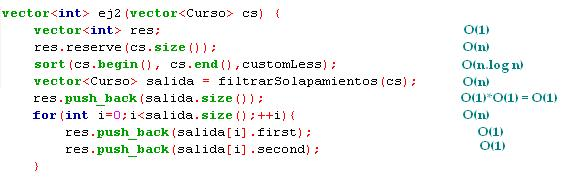
\includegraphics[width=0.7\textwidth]{../imgs/comple2.jpg}
% \end{center}
% \end{figure}

% Finalmente, la complejidad es: $\mathcal{O}(1)+\mathcal{O}(n)+\mathcal{O}(n\ log\ n)+\mathcal{O}(n)+\mathcal{O}(1)+\mathcal{O}(n)*\mathcal{O}(1)*\mathcal{O}(1)$ = \textbf{\mathcal{O}(n\ log\ n)}

\subsection{Código fuente}



\subsection{Instancias posibles}

Para verificar la correctitud de nuestro programa, dispusimos variar estratégicamente las instancias de entrada al ejecutarlo.
\begin{itemize}
\item En primer lugar, decidimos mostrar un caso en el que no se solapara ningún curso. En esta ocasión, puede observarse que, dado que hay una solución óptima, ésta es única. De este modo, se logra verificar que los cursos de la entrada coinciden con los de la salida.\newline
\textbf{Parámetro de entrada:} $$3\ \ 0\ \ 1\ \ 3\ \ 5\ \ 6\ \ 9$$
\textbf{Parámetro de salida:} $$3\ \ 1\ \ 2\ \ 3$$\newline


\begin{figure}[H] %[h] Aqui [b] para button [t] para top
\begin{center}
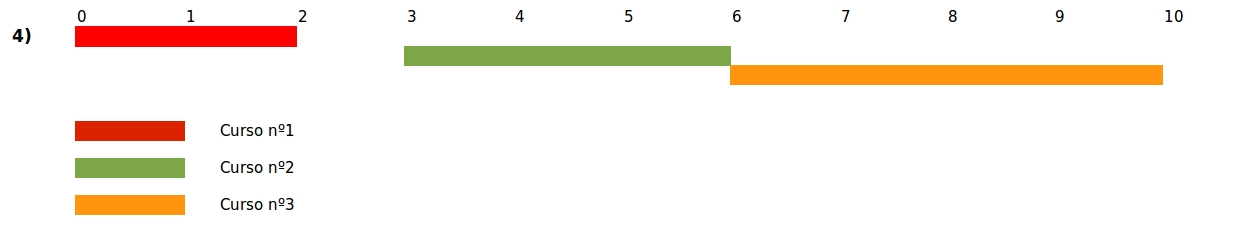
\includegraphics[width=450pt]{../imgs/instancia4.jpg}
\end{center}
\caption{Instancia posible nº1.}
\end{figure}

\item Por otra parte, probamos el programa para la situación en la que no se ingresa ningún curso. Esto sería, por lo tanto, el caso vacío. Dado que este caso borde es muy significativo, nos pareció interesante mencionarlo.\newline
\textbf{Parámetro de entrada:} $$0$$
\textbf{Parámetro de salida:} $$0$$ \newline


\item Otro caso a considerar es en el que todos los cursos finalizan el mismo día (solapándose todos entre sí). Debido a que cualquiera de ellos es solución del problema pues es la máxima cantidad de intervalos que no se solapan, utilizamos esta instancia para verificar que nuestro algoritmo devolviera siempre el de menor fecha de finalización. \newline
\textbf{Parámetro de entrada:}  $$3\ \ 1\ \ 5\ \ 3\ \ 5\ \ 2\ \ 5$$
\textbf{Parámetro de salida:}  $$1\ \ 1$$\newline

\begin{figure}[H] %[h] Aqui [b] para button [t] para top
\begin{center}
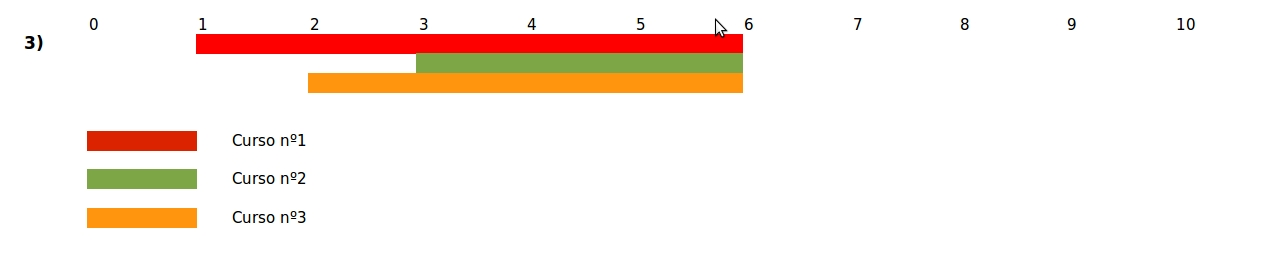
\includegraphics[width=450pt]{../imgs/instancia3.jpg}
\end{center}
\caption{Instancia posible nº3.}
\end{figure}


\item Por último, consideramos interesante considerar el caso en el que existe al menos un curso que se solapa. Dicho caso sería el más común en el problema a resolver. Este tipo de situaciones tienen más de una solución óptima. En esta oportunidad, hay dos salidas posibles que son solución del problema. Debido que nuestro algoritmo almacena, en primer lugar, los intervalos cuya fecha de fin es la más alta, dicho intervalo es el prioritario frente a cualquiera que se le solape. Del mismo modo, decidimos que podía ser interesante considerar el caso de cursos cuya fecha de inicio fuera igual a la fecha de fin para comprobar que las cotas del programa estuvieran definidas correctamente.\newline
\textbf{Parámetro de entrada:}  $$4\ \ 0\ \ 3\ \ 3\ \ 5\ \ 7\ \ 10\ \ 8\ \ 9$$
\textbf{Parámetro de salida:}  $$2\ \ 1\ \ 4$$ \newline

\begin{figure}[H] %[h] Aqui [b] para button [t] para top
\begin{center}
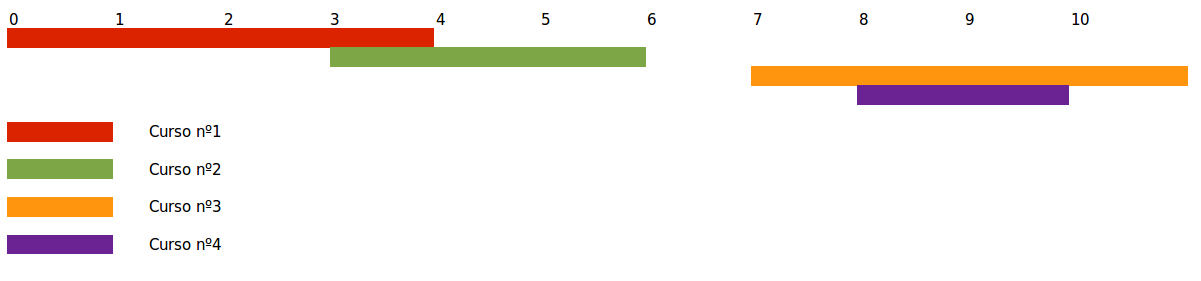
\includegraphics[width=450pt]{../imgs/instancia1.jpg}
\end{center}
\caption{Instancia posible nº4.}
\end{figure}

\end{itemize}

\subsection{Testing}
